\section{Framework Overview}
\ek{Need to add the workshop terminology and characteristics before this section.}
\label{sec:overview}

The framework consists of two models for analyzing creativity workshops in the early stages of visualization design work: 1) a workshop process model that describes the commonly repeated actions and decisions of researchers using workshops; and 2) a workshop design model that describes a general structure through which creativity methods can be flexibly applied in conducting such workshops. These models are shown in Fig.~\ref{fig:cascading-process} and summarized in this section.

\subsection{Process Model}

Analyzing the process of workshops is challenging as they can be used for a variety of reasons, including to identify key aims for funded collaboration [\ref{wor:arbor}], to explore visualization opportunities within a collaboration [\ref{wor:eon},\ref{wor:htva}], or to examine specific domain tasks [\ref{wor:lineage}]. In these cases, a three-stage process model can abstract and describe the actions performed before, during, and after a workshop. The stages are completed with forward linear movement, and upstream decisions cascade downstream.

The model starts with \emph{decide \& design}, in which we decide to use a workshop and decide on its intended outcome, length, venue, participants, and facilitators. We also design the workshop methods to achieve the intended outcome, but this can change our understanding of the domain, causing us to revisit decisions about the workshop's intended outcome, participants, etc. This stage results in a flexible \emph{workshop plan} outlining methods we intend to use in the workshop, and resolving practical concerns, such as the duration, venue, materials, and participants.

The second stage is \emph{execute \& adapt}, in which we perform the workshop plan while adapting it to the emergent understanding of visualization and data analysis opportunities as well as participant reactions. This stage results in \emph{workshop output}, a set of rich and descriptive artifacts, participant feedback, and notes documenting experiential knowledge. 

The third stage is \emph{analyze \& act}, in which we analyze workshop output, creating insights that we act on throughout the design process. Analysis and action are mutually influential as we learn through action and reanalyze workshop output with this new knowledge. This stage results in actionable knowledge integrated into the design process, for example, through generative and evaluative design methods. 

This model is particularly relevant to visualization as it recognizes that: 1) designing a workshop influences our understanding of domain-relevant opportunities for visualization; 2) executing a workshop enables us to adapt it to explore emergent (research) problems; and 3) analyzing workshop output influences visualization design decisions. These nuances are not addressed in other models, such as a process for educational workshops of \emph{pre-design, design, facilitation, and action}~\cite{Brooks-Harris1999}, as well as a process for business workshops of \emph{plan, perform, and act}~\cite{Hamilton2016}. Furthermore, we support this model with 19 actionable recommendations for future workshops, described in Sec.~\ref{sec:recommendations}.

\subsection{Design Model}

Analyzing the methods used in workshops is challenging because workshops are diverse --- they can be used for a variety of reasons, they can range in length from a few hours [\ref{wor:lineage}] to two days [\ref{wor:arbor}], and they can involve a variety of participants, including collaborators who regularly work together [\ref{wor:eon}], a mix of visualization researchers and collaborators [\ref{wor:htva}], or a set of practitioners, educators, and students [\ref{wor:cp}]. Despite all the factors that influence workshop methods, we propose a three stage \emph{workshop design model} that describes many of the successful creativity workshops with which we have been involved. It supports analysis of methods used in the beginning, during the middle, or at the end of workshops. The stages of this model are also completed in a forward linear fashion and have cascading effects on the workshop design and thus execution. 

% While the process model examines the actions of researchers, the design model arises from analysis of workshop methods. And, they can be used for different purposes, as described above. Thus, we frame decisions about workshop methods as a design problem because there is not a single `correct' workshop, that there is no exhaustive list of possible workshops, and that workshop effectiveness depends on its context and intended outcomes. 

The model starts with a \emph{workshop opening} that can communicate why the workshop is being run and establish an atmosphere conducive to productivity and creativity. Next, the \emph{workshop core} can promote group creativity and exploration of emergent ideas. Finally, the \emph{workshop closing} can conclude the workshop, providing validation, as well as a sense of achievement and agreement over next steps.

Unlike the process model, the design model stages are open to interpretation. For example, the workshop opening could be interpreted as the first two minutes, the first two hours, or the first two methods --- these are all valid. There are no crisp boundaries between stages as the model identifies general characteristics of workshop methods in the opening, the core, and the closing. \new{Although we provide an illustrative example workshop} \rem{In fact}, we emphasize the need for creativity workshops to be flexible in response to participants knowledge, reactions, activity, discovery, outputs and energy, and diverse in terms of the types of method employed. Furthermore, effective workshops will smoothly transition between the three stages.

At a high-level of abstraction, the design model resembles existing workshop theory as characteristics of harnessing group creativity are domain-independent. For example, similar design models appear in: the \emph{gamestorming} framework which describes workshop-like games in three stages of open, explore, and close~\cite{Macanufo2010}; an educational workshop framework that separates the introduction, learning activities, and conclusion~\cite{Brooks-Harris1999}; and Creative Problem Solving that distinguishes between a beginning (to clarify the problem), a middle (to ideate and develop solutions) and a conclusion (to formulate a plan for action)~\cite{CreativeEducationFoundation2015}. While these similarities validate our model, we support it with 17 actionable design considerations for selecting methods particularly useful for visualization research, described next.

\begin{figure}
    \centering
    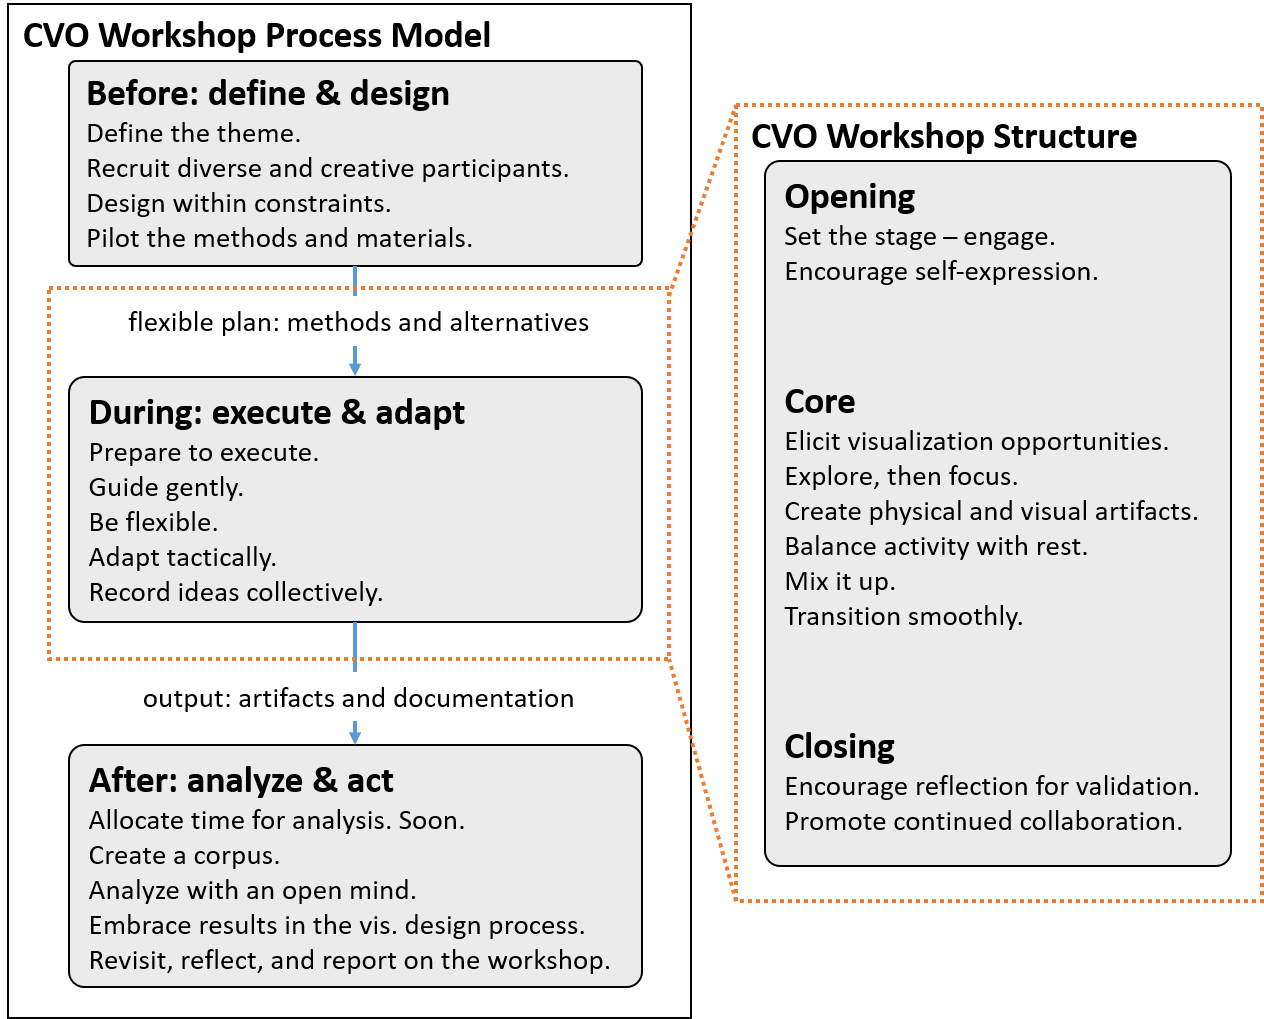
\includegraphics[width=0.8\columnwidth]{figures/framework-overview.png}
    \caption{\ek{Placeholder! Any suggestions to make this more compelling?} The visualization creativity workshop framework consists of a process model to describe the actions of researchers using workshops (left), and a design model to describe the workshop methods (right).}
    \label{fig:cascading-process}
\end{figure}

% We propose a process model to abstract and simplify the actions of researchers into six stages that are conducted in a forward, linear fashion, as shown in Fig.~\ref{fig:cascading-process}. It starts with \emph{initialization}, deciding to use a workshop, articulating its purpose, identifying its constraints (e.g., duration, venue, budget), inviting participants, and recruiting team members. The output from initialization is defined broadly as the \emph{workshop context}. The context influences the \emph{design}, selecting and fine-tuning workshop methods for its intended purpose. The output from design is a flexible \emph{workshop plan} that describes the workshop methods. The plan is carried out during \emph{execution}, performing the workshop methods. This results in artifacts and experiential knowledge which we make sense of during \emph{analysis}. The results of analysis are integrated into the collaboration through \emph{action}. Permeating the process is \emph{reflection}, as we review our experiences to generate insights. 

% The model is cascading as decisions upstream propagate to downstream stages. For example, reason for running a workshop influences the methods that may be effective, and the methods influence the workshop output. The model is also iterative as knowledge gained from downstream stages necessitates revisiting those upstream. While we are selecting workshop methods, we test and improve our understanding of the domain which can the workshop context and its intended outcome. Similarly, action on the workshop results generates new knowledge that can influence continued analysis of workshop artifacts. Details on the iterative movement between workshop stages is discussed in Sec.~\ref{sec:recommendations}.

% A set of design considerations for selecting workshop methods supports the process model. The considerations can be considered context-independent as workshops with similar methods can be reused between projects (e.g., [\ref{wor:eon}, \ref{wor:graffinity}]). But they are also context-dependent, as reusing workshop methods requires fine-tuning them based on, for example, the collaborator's data. We describe the design considerations next to provide an understanding of what happens during workshops and to establish concepts for reflective analysis of the workshop process. 



%but While the action of designing workshops is contained within the model, there are decisions made in designing a workshop that are context-independent. An important goal of creativity workshops is that they promote synergistic group creativity, characterized by focused work, open communication, exploration, revisiting of ideas~\cite{Sawyer2003}. Considerations for workshop methods that support group creativity are context-independent. Thus, we have separated the workshop design considerations from the workshop process. Aspects of the design considerations, however, account for the customization of workshop methods to specific contexts---such as the goals of the project, the experience of researchers, and challenges of domain-specific data.

%The workshop design also cascades through the workshop process. The workshop methods define what artifacts are generated, and this influences the possibilities to analyze the artifacts and act on the results of that analysis. Thus, we introduce the workshop design considerations before describing our detailed analysis, reflections, and recommendations supporting the workshop process. 

%To understand how and why to use creativity workshops in applied visualization, we initially reflected on three workshops that used similar methods---examining details such as the venue, the participants, the duration of methods, and the artifacts that they produced. We were able to connect workshop methods to artifacts and evaluate their influence on generative and evaluative methods, but this analysis was too narrowly scoped. We could not account for the different reasons for running the workshops, such as to explore far-reaching future technologies [\ref{wor:eon}], to expose shared needs from diverse workflows [\ref{wor:graffinity}], and to quickly establish a domain problem characterization [\ref{wor:cp}]. We also struggled to analyze workshops that used different methods (e.g., [\ref{wor:eon}, \ref{wor:htva}]), and concluded that the workshop methods did not provide enough information to gain a detailed understanding. 

%After months of floundering, reviewing literature, discussing past experiences, and ideating, we tried analyzing workshops from the perspectives of educational workshops~\cite{Brooks-Harris1999}, creative problem solving~\cite{CreativeEducationFoundation2015}, and various others~\cite{DeBono1983,Gordon1961,Stanfield2002}. Although these perspectives could not account for the nuances of visualization design, such as the importance of data and the use of specialized process models, they generally used a common dimension for describing workshops: time. Although workshops can vary on many attributes --- methods, participants, purpose, outcomes, etc. --- they tended to follow a process that required specific actions and decisions before, during, and after the workshop. The process of using a workshop became the foundation for our analysis as we proposed a model that provided a vocabulary to talk about the cascading influence of reasons for running a workshop, the methods used in the workshop, and the actions based on workshop output.

%The process allowed us to compare and contrast different workshop experiences, and we discovered important ideas about how and why to use workshops. But this analysis confounded the actions performed by researchers (in the context of the collaboration) with the actions performed by participants (in the context of the workshop). It was challenging to analyze the actions of researchers in projects that used different workshop methods as the two were closely linked in the process model. We separated decisions about what methods to use in a workshop from the workshop process in order to support analysis of workshop methods independent of the larger context of the collaboration, potentially supporting the reuse of workshops between diverse projects and simplifying the presentation of our model. 

%The resulting visualization creativity workshop framework consists of a cascading process model and a series of design considerations. The process starts with \emph{initialization} where we decide to whether to use a creativity workshop. If so, we then \emph{design} the workshop by selecting appropriate methods. Design is followed by \emph{execution}, performing the workshop and collecting artifacts. Next, during \emph{analysis}, we make sense of the workshop outputs, creating knowledge. This knowledge is integrated into the project through \emph{action}. Permeating the process is \emph{reflection}, as we review our experiences to generate insights. Stages of the process are completed in a cascading, linear fashion. Decisions from upstream stages cascade to downstream stages. For example, the reason for initializing a workshop influences the appropriate design. As the model represents complex and messy actions of researchers, it also describes the cyclical influence between stages. For example, designing a workshop can reveal valuable insights on why a workshop is being run. Similarly, acting on the workshop results can generate new knowledge that influences how workshop results are analyzed. The model is also nested as it is carried out by researchers who learn from the experiences and actions. 

%The framework's design considerations a series of thinking tools for understanding the methods used in a workshop at different levels of abstraction. They support the analysis of our past workshops, enabling us to understand where methods may be appropriate to use in a workshop. They also provide guidance on how to account for the context of the collaboration, such as the relevant data, tasks, or automation. Next, we describe the design considerations, but we recognize that they a part of the larger process...


%We propose a six stage process model for creativity requirements workshops in applied visualization research projects, as shown in Fig.~\ref{fig:cascading-process}. The process starts with \emph{initialization} where we decide to whether to use a creativity workshop. If so, we then \emph{design} the workshop by selecting appropriate methods. Design is followed by \emph{execution}, performing the workshop and collecting artifacts. Next, during \emph{analysis}, we make sense of the workshop outputs, creating knowledge. This knowledge is integrated into the project through \emph{action}. Permeating the process is \emph{reflection}, as we review our experiences to generate insights. Stages of the process are completed in a cascading, linear fashion. Decisions from upstream stages cascade to downstream stages. For example, the reason for initializing a workshop influences the appropriate design. As the model represents complex and messy actions of researchers, it also describes the cyclical influence between stages. For example, designing a workshop can reveal valuable insights on why a workshop is being run. Similarly, acting on the workshop results can generate new knowledge that influences how workshop results are analyzed. The model is also nested as it is carried out by researchers who learn from the experiences and actions. This section summarizes each stage of our workshop process.

%Workshop \emph{initialization} leads to the decision as to whether to run a workshop.

%Next, workshop \emph{design} is about creating a flexible workshop plan that identifies methods to be used during the workshop tailored to the appropriate context. We emphasize that design creates a flexible plan because the output of methods ultimately depends on how they are received by the participants during execution. We describe the details of workshop design in Sec.~\ref{sec:design}.

%After design, the workshop is run during \emph{execution}. Execution is a performance: the workshop team continuously adapts to the feedback from workshop participants. \jd{I think you need `effective` in here, which means that later we need evidence to support our claim} Effective execution requires deviating from the plan in ways that are both profound and subtle. It results in a plethora of workshop artifacts and documentation, tangible results created through the workshop methods or recorded by the workshop team.

%We make sense of the workshop results during \emph{analysis}. Performed by the workshop team, it involves identifying insights in the form of themes, patterns, key concepts, or outliers from the workshop artifacts. 

%The knowledge gleaned from workshop analysis influences the workshop \emph{action}, where we continue the collaboration. This includes the action of visualization researchers as the workshop provides new information valuable for generative and evaluative design methods. It also includes the workshop participants as they may approach existing problems or practices in a new way.  

%Permeating the process is \emph{reflection}, where we generate knowledge from experience. We reflect on our experience executing the workshop, on the effectiveness of workshop design, on the influence of workshop results on the project’s outcomes, and on the use of workshops in different projects and contexts.

%Although this model simplifies the complex actions of researchers, it provides a consistent vocabulary for us to connect our actions with their intended outcome across diverse projects. This model serves as a roadmap for researchers to apply workshops in their own project. We augment this roadmap with a series of actionable recommendations (see Sec.~\ref{sec:recommendations}). Next, we describe a set of thinking tools for navigating the possible design space of workshops. 